\documentclass[11pt,a4paper]{article}
\usepackage[margin=2cm]{geometry}
\usepackage[T1]{fontenc}
\usepackage{lmodern}
\usepackage{microtype}
\usepackage{amsmath}
\usepackage{graphicx}
\usepackage{booktabs}
\usepackage{tabularx}
\usepackage{enumitem}
\usepackage{xcolor}
\usepackage{caption}
\usepackage{titlesec}
\usepackage[section,above]{placeins}
\usepackage[hidelinks]{hyperref}

\graphicspath{{../outputs/figures/}}
\definecolor{accent}{HTML}{1C5CAB}
\titleformat{\section}{\large\bfseries\color{accent}}{\thesection.}{0.5em}{}
\titleformat{\subsection}{\normalsize\bfseries}{\thesubsection}{0.5em}{}
\titlespacing*{\section}{0pt}{10pt}{4pt}
\titlespacing*{\subsection}{0pt}{6pt}{2pt}
\setlist{nosep, leftmargin=1.3em}
\captionsetup{font=small, labelfont=bf, skip=3pt}
\setlength{\parskip}{3pt}
\setlength{\parindent}{0pt}
\setlength{\textfloatsep}{8pt}

\begin{document}

{\centering
{\LARGE\bfseries Assignment 1: Opinion Network Formation}\\[4pt]
{\large DPCN}\\[2pt]
{\normalsize Inesh \quad$\cdot$\quad Khwaish \quad$\cdot$\quad Hiten}\\[2pt]
{\small September 2026}\par}
\vspace{6pt}

\section{Team Name}
\textbf{Team KHI} (Khwaish, Hiten, Inesh).

\section{GitHub Link to Our Code}
\url{https://github.com/iDheer/KHI}\\
The repository holds the raw data (\texttt{data/}), the modular source code in \texttt{src/}
(\texttt{preprocess.py}, \texttt{network.py}, \texttt{analysis.py}, \texttt{visualize.py}), a single entry point
(\texttt{python run\_pipeline.py}) that regenerates every table, figure and metric in this report in
$\approx$30\,s, the exported networks in GraphML (\texttt{outputs/}) and this report's \LaTeX{} source.
All random steps are seeded, so the results are fully reproducible.

%==============================================================================================
\section{Dataset Documentation}
\subsection{What the survey contains}
The export \texttt{Survey\_Results\_UC.csv} has one row per submission and 61 columns: a response
ID and 60 Likert statements, 15 per theme -- \textbf{Technology} (T01--T15, e.g.\ AI, automation,
privacy, regulation), \textbf{Education} (E01--E15, e.g.\ exams, attendance, online and project-based
learning), \textbf{Ethics \& Society} (S01--S15, e.g.\ accountability, inclusion, misinformation) and
\textbf{Environment} (V01--V15, e.g.\ climate action, plastics, sustainability). Every statement offers
five ordered options plus a ``No Comments'' option. The file contains \textbf{96 submissions}; their IDs
run from 11 to 126 but are not consecutive (IDs 1--10 and 20 others never appear), so the largest ID should
not be mistaken for the number of respondents.

\subsection{Interpretation and preparation}
\begin{enumerate}
\item \textbf{Encoding.} Answers were mapped to an ordinal scale:
Strongly Disagree $=-2$, Disagree $=-1$, Neutral $=0$, Agree $=+1$, Strongly Agree $=+2$.
The symmetric scale makes ``0'' mean ``no position'' and the sign mean direction. The script
fails loudly if any unexpected label appears.
\item \textbf{``No Comments'' is missing, not neutral.} Declining to answer is different from sitting on the
fence, so the 37 ``No Comments'' answers were set to missing rather than 0. Blank cells were treated the same way.
\item \textbf{Quality filtering.} We counted the answered statements per respondent. \textbf{5} rows were
completely empty and \textbf{4} rows answered only the 15 Technology statements (the rest of the form was
abandoned). A respondent was kept only if they answered $\geq$75\% (45/60) of the statements, which leaves
\textbf{87 respondents}. Two kept respondents are partial (\#79 skipped Environment, \#123 skipped 10
statements); 62 of the 5{,}220 retained cells (1.2\%) are missing.
\item \textbf{No imputation.} Missing values are handled pairwise (Section~4), so no answers were invented.
\item \textbf{Checks for bad-faith responses.} No kept respondent gave the same answer to all 60 statements
(the most uniform used one label for 87\% of answers but still used 5 different labels), and no two
respondents were exact duplicates. Nobody was removed on these grounds.
\end{enumerate}

\subsection{First look at the answers}
The class agrees with most statements: \textbf{79.1\%} of all answers are Agree or Strongly Agree
(42.9\% Strongly Agree) and only 7.0\% are negative; the mean score is $+1.14$. Environment ($+1.39$)
and Ethics \& Society ($+1.28$) get the strongest support, Technology ($+1.00$) and Education ($+0.91$)
the weakest. To tell real disagreement apart from a simple difference in averages we used the
\emph{Tastle--Wierman consensus} $\mathrm{Cns}=1+\sum_i p_i\log_2\!\left(1-|x_i-\mu|/4\right)$, which is 1 when
everyone answers the same and 0 when the class splits between the two extremes (Fig.~\ref{fig:dist}, bottom).
The most \emph{divisive} statements are all about teaching practice or AI in practice: online learning as a
complement to classroom teaching (E04, 54\% agree vs.\ 28\% disagree, Cns $=0.55$), written exams as an
accurate measure (E02, 32\% vs.\ 43\%), compulsory attendance (E03, 70\% \emph{disagree}) and routine
AI diagnosis in healthcare (T08). The most \emph{consensual} are lifelong learning (E15, Cns $=0.83$),
corporate environmental accountability (V13) and personal control over data (S05).

\begin{figure}[t]
\centering
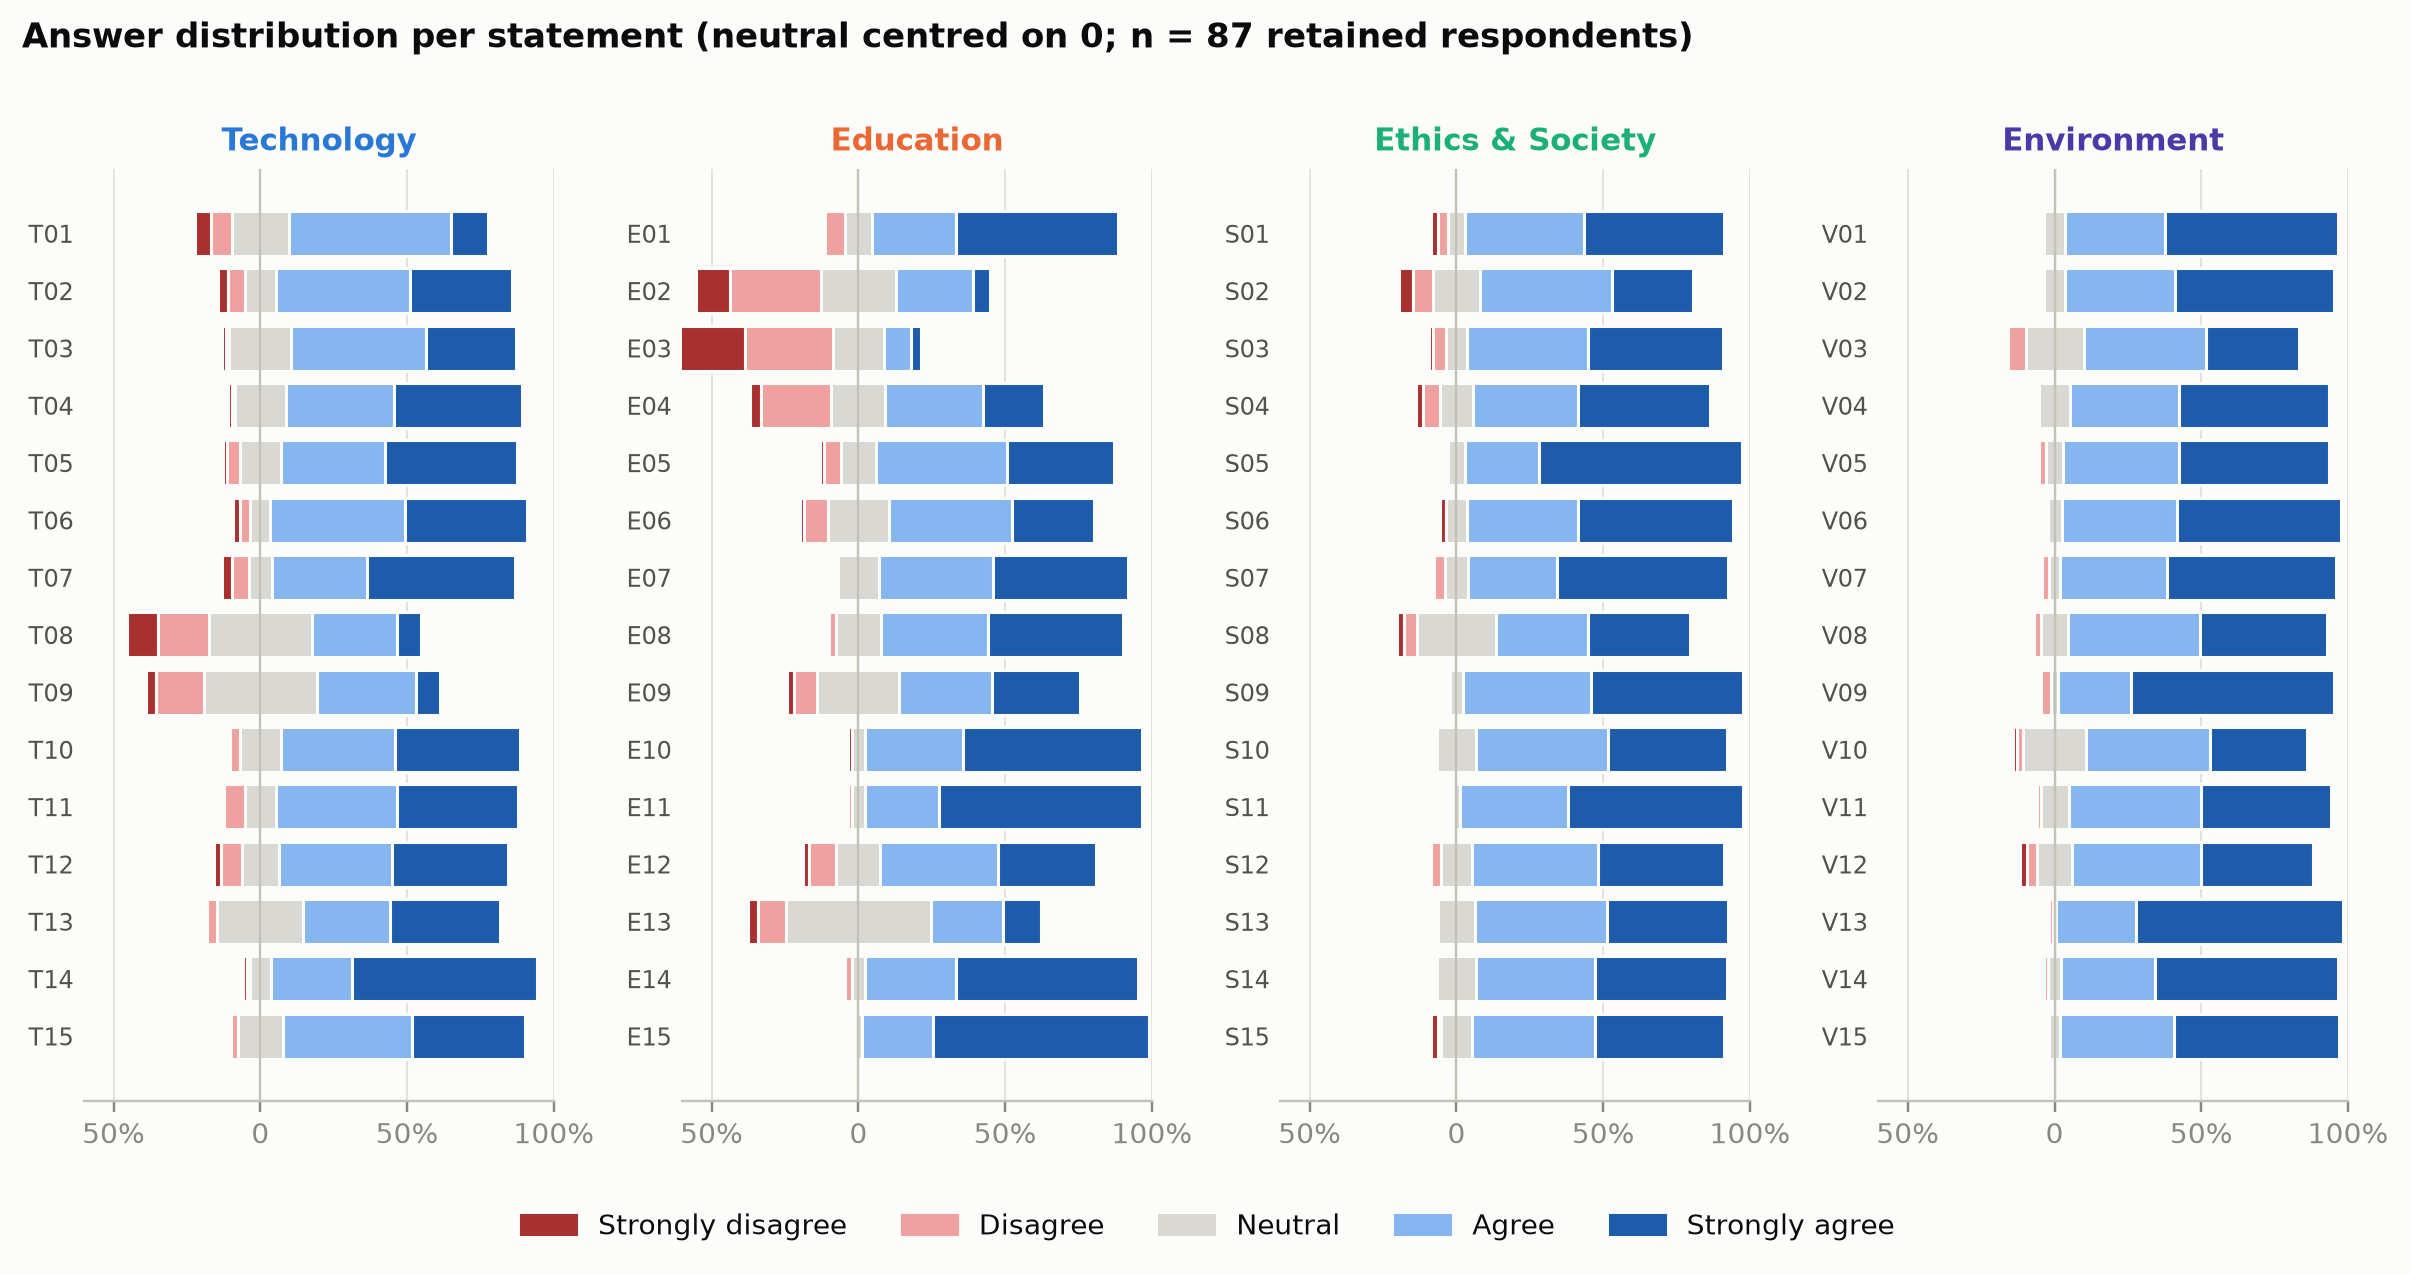
\includegraphics[width=\linewidth]{fig01_response_distribution.png}\\[2pt]
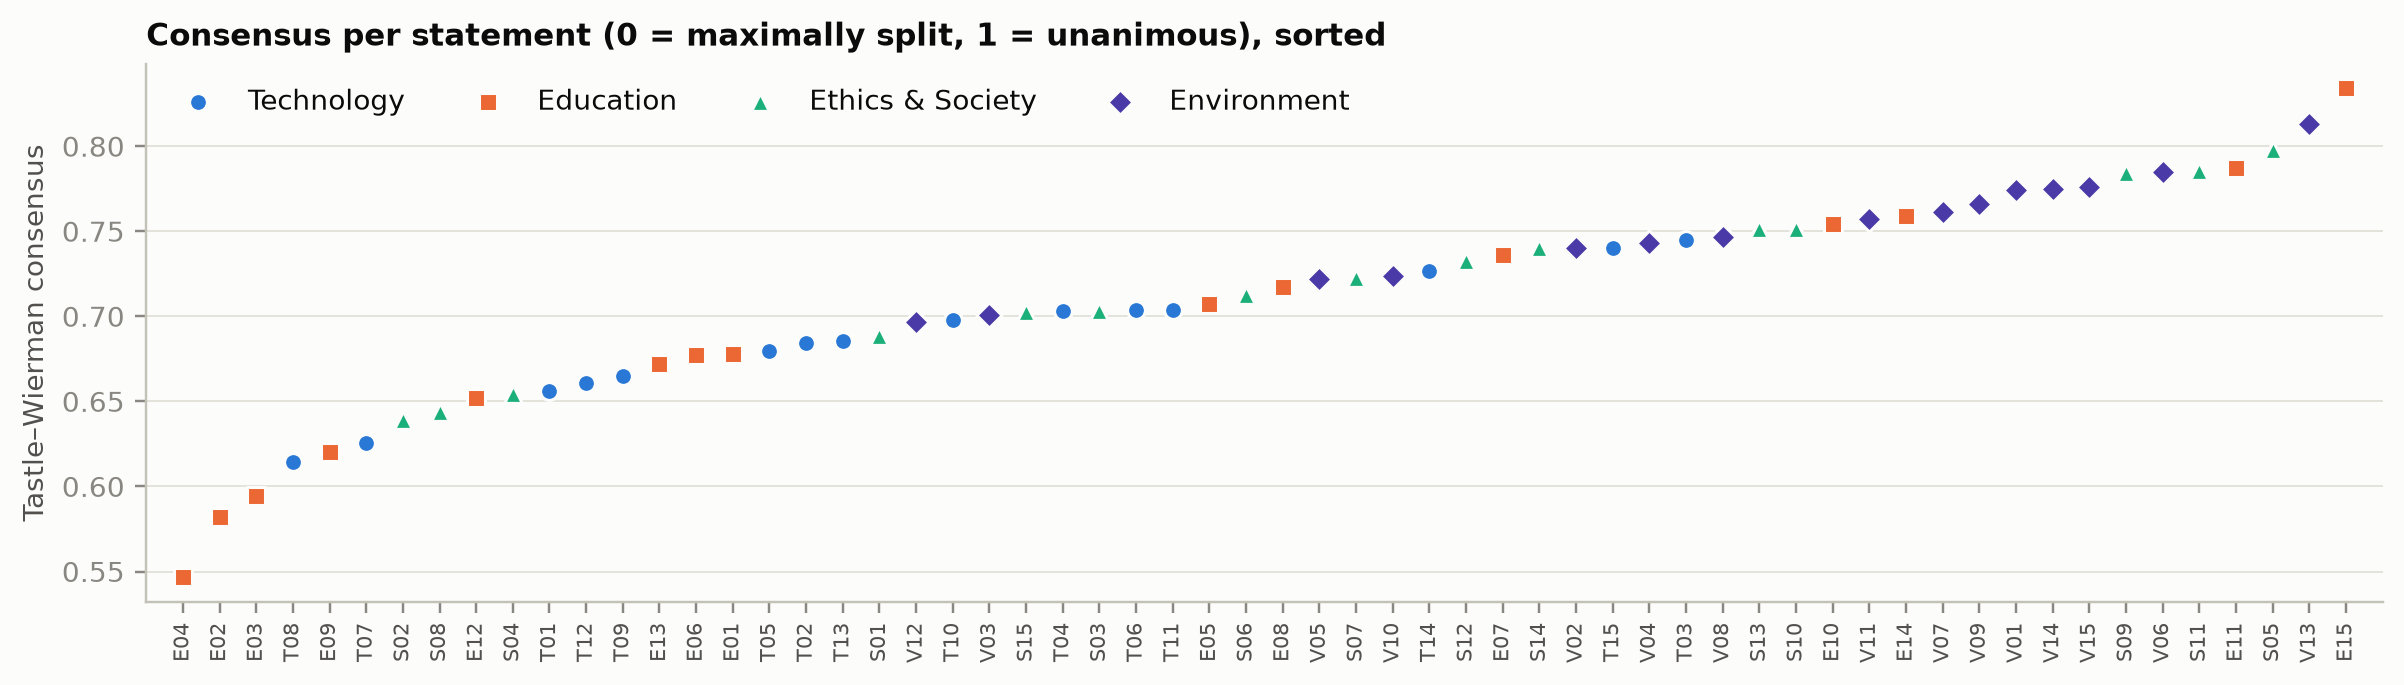
\includegraphics[width=\linewidth]{fig02_consensus.png}
\caption{Top: answer distribution per statement. Each bar is split at the middle of ``Neutral'', so
disagreement extends left and agreement right. Bottom: Tastle--Wierman consensus per statement; colour and
marker show the theme.}
\label{fig:dist}
\end{figure}

%==============================================================================================
\section{Pipeline Followed}
We build \textbf{two complementary networks} from the same response matrix
$X\in\{-2,\dots,2\}^{87\times60}$:
\begin{itemize}
\item a \textbf{respondent network} (the main object): nodes are students, and an edge means two students hold
\emph{similar opinion profiles}. Its communities are ``opinion groups'';
\item a \textbf{statement network}: nodes are the 60 statements, and an edge means students answer the two
statements \emph{in the same way}. Its communities reveal which opinions go together.
\end{itemize}

\subsection{Respondent network}
\begin{enumerate}
\item \textbf{Item centring.} Because nearly everyone agrees with most statements, raw answer vectors all
point the same way and every pair of students looks alike (in our tests, raw cosine similarity gives
almost no community structure, $Q=0.26$). We therefore subtract each statement's class mean:
$z_{ij}=x_{ij}-\bar x_{\cdot j}$. Two students are now similar when they \emph{deviate from the class
consensus in the same direction}.
\item \textbf{Pairwise-complete cosine similarity.}
$s_{uv}=\frac{\sum_{j\in J_{uv}} z_{uj}z_{vj}}{\sqrt{\sum_{j\in J_{uv}} z_{uj}^2}\sqrt{\sum_{j\in J_{uv}} z_{vj}^2}}$
where $J_{uv}$ contains the statements both students answered (at least 30 required). Similarities are
centred on 0 (mean $-0.01$, SD $0.20$, 5th--95th percentile $[-0.33,\,0.32]$; Fig.~\ref{fig:construction}a).
\item \textbf{Sparsification into a $k$-nearest-neighbour backbone.} A complete weighted graph is not
informative, and a global threshold would leave students with unusual views isolated. Each student is
linked to its $k$ most similar peers (only positive similarities), and the result is made symmetric:
an edge $u$--$v$ exists if either student is in the other's top-$k$. Edge weight $=s_{uv}$.
\item \textbf{Choosing $k$.} We tried $k=2,\dots,15$ (Fig.~\ref{fig:construction}b--c). Small $k$ splits the graph
into many small groups with inflated modularity. From $k=8$ on, the number of communities settles at
2--3, the modularity curve flattens and partition stability rises again. We therefore use \textbf{$k=8$},
the smallest value in this stable range.
\item \textbf{Community detection.} We ran weighted Louvain modularity optimisation with 100 random seeds, kept the
partition with the highest modularity, and measured stability as the mean Adjusted Rand Index (ARI) between
that partition and all 100 runs.
\item \textbf{Validation.} (i) \emph{Permutation null model:} we shuffled each statement's column independently
200 times. This keeps every statement's answer distribution but breaks the link between a person's answers.
Each shuffled dataset went through the same pipeline. (ii) \emph{Degree-preserving rewiring}
(50 double-edge-swap graphs) for clustering and path length. (iii) \emph{Construction robustness:} we compared
the partitions from other values of $k$, a global top-10\% threshold graph, person-centred cosine and uncentred cosine.
(iv) \emph{Resolution sweep} of Louvain, $\gamma\in[0.6,2]$.
\item \textbf{Profiling.} For each statement, a Kruskal--Wallis test across communities (effect size
$\eta^2_H=(H-k+1)/(n-k)$, Benjamini--Hochberg FDR) identifies what separates the groups. We also computed
degree, strength, weighted clustering, betweenness and closeness (on distance $1-s$) and eigenvector centrality.
\item \textbf{Per-theme networks.} We repeated steps 1--5 using only one theme's 15 statements and compared the
four resulting partitions with ARI, to test whether students who group together on one topic also group together on the others.
\end{enumerate}

\subsection{Statement network}
\begin{enumerate}
\item We computed the Spearman rank correlation $\rho$ for all $\binom{60}{2}=1{,}770$ statement pairs (pairwise complete; Spearman suits ordinal data).
\item We kept an edge only if the correlation was significant after Benjamini--Hochberg FDR correction ($q<0.05$) \emph{and} $\rho\geq0.30$,
with weight $\rho$. Significant negative correlations ($\rho\leq-0.30$) are too few to form a signed network (6 pairs), so we report them separately.
\item We ran Louvain (100 seeds) and compared the detected communities with the four questionnaire themes using NMI and ARI.
\end{enumerate}

\begin{figure}[t]
\centering
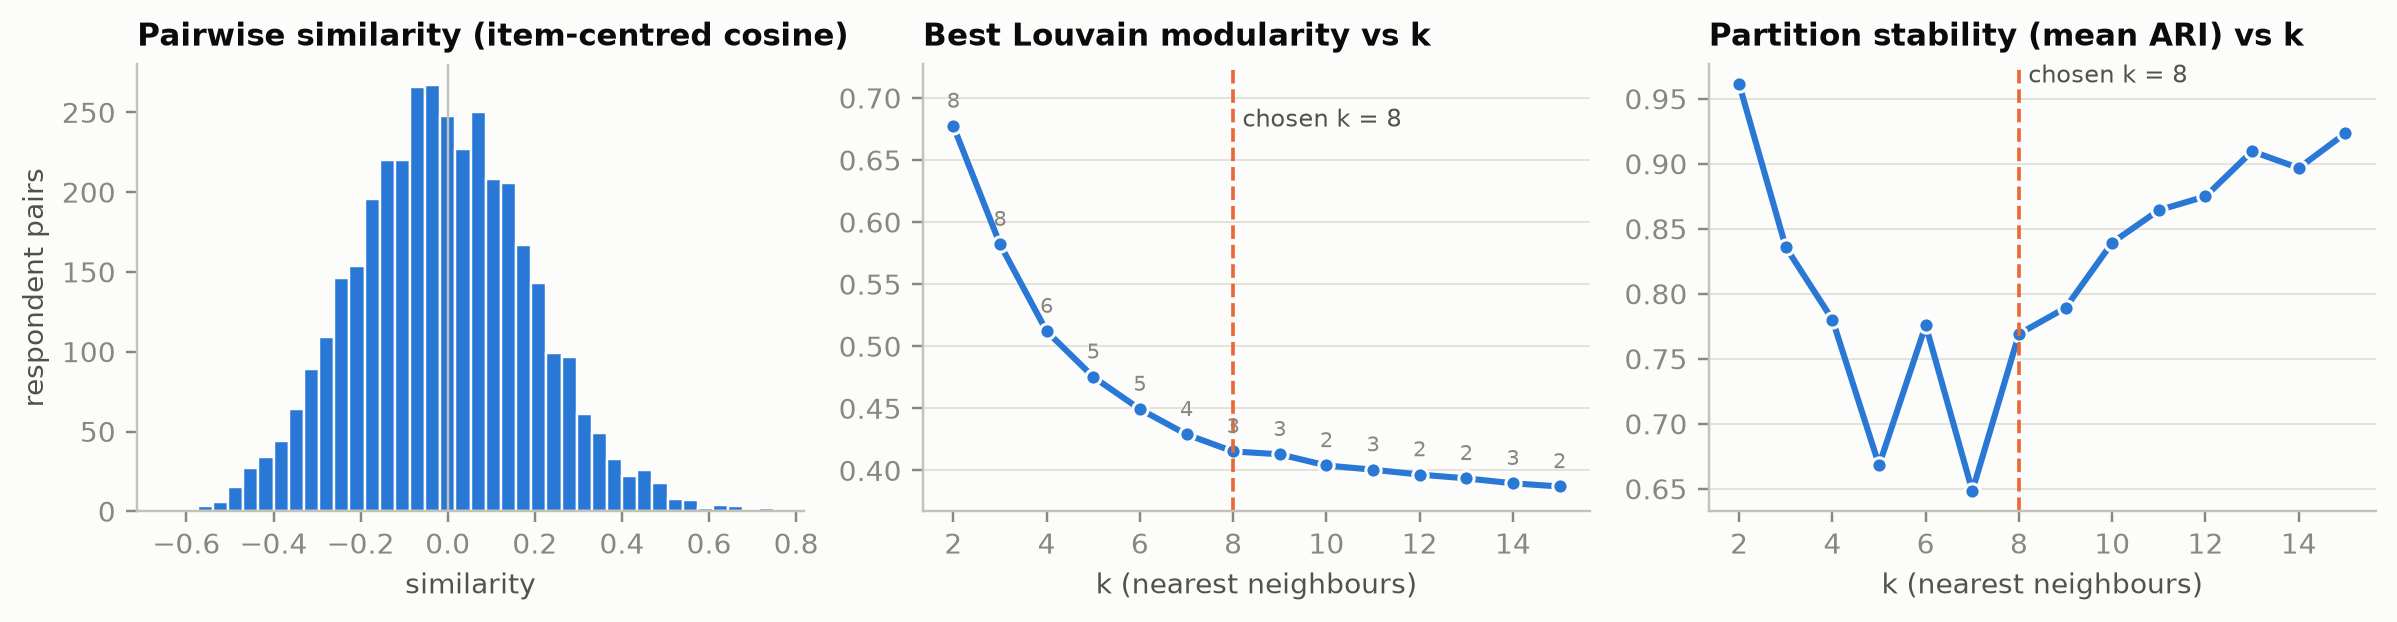
\includegraphics[width=\linewidth]{fig03_construction.png}
\caption{Construction diagnostics. (a) Distribution of item-centred similarities. (b) Best Louvain modularity
vs.\ $k$ (numbers show the community count). (c) Mean ARI of 20 Louvain runs vs.\ $k$.}
\label{fig:construction}
\end{figure}

%==============================================================================================
\clearpage
\section{Analysis and Visualizations}
\subsection{Respondent network: global metrics}
\begin{table}[h]
\centering\footnotesize\setlength{\tabcolsep}{3pt}
\begin{tabular}{@{}lr@{\hspace{10pt}}lr@{\hspace{10pt}}lr@{}}
\toprule
Nodes & 87 & Degree mean (min/max) & 10.7 (8/20) & Transitivity (rewired) & 0.31 (0.12$\pm$0.01)\\
Edges & 466 & Mean edge weight & 0.314 & Mean path (rewired) & 2.31 (2.10)\\
Density & 0.125 & Avg.\ clust.\ (weighted) & 0.286 (0.129) & Small-world $\sigma$ & 2.26\\
Components & 1 & Degree assortativity & $+0.10$ & Diameter & 4\\
\midrule
Communities & 3 (45/23/19) & Modularity $Q$ & 0.418 & Seed stability (ARI) & 0.74\\
Null $Q$ (shuffled) & 0.363$\pm$0.014 & $z$-score / $p_{\text{emp}}$ & 4.0 / 0.005 & Differing stmts ($q<.05$) & 49 of 60\\
\bottomrule
\end{tabular}
\caption{Key metrics of the respondent opinion network ($k=8$).}
\label{tab:metrics}
\end{table}

The network is connected and has \emph{small-world} structure. Its clustering is 2.5$\times$ higher than in
degree-preserving random graphs, while paths are only 10\% longer ($\sigma=2.26$). Students who share a
like-minded peer tend to be like-minded themselves, so groups form, yet any two students are at most 4 steps apart.
Degree assortativity is weakly positive (0.10).

\begin{figure}[!h]
\centering
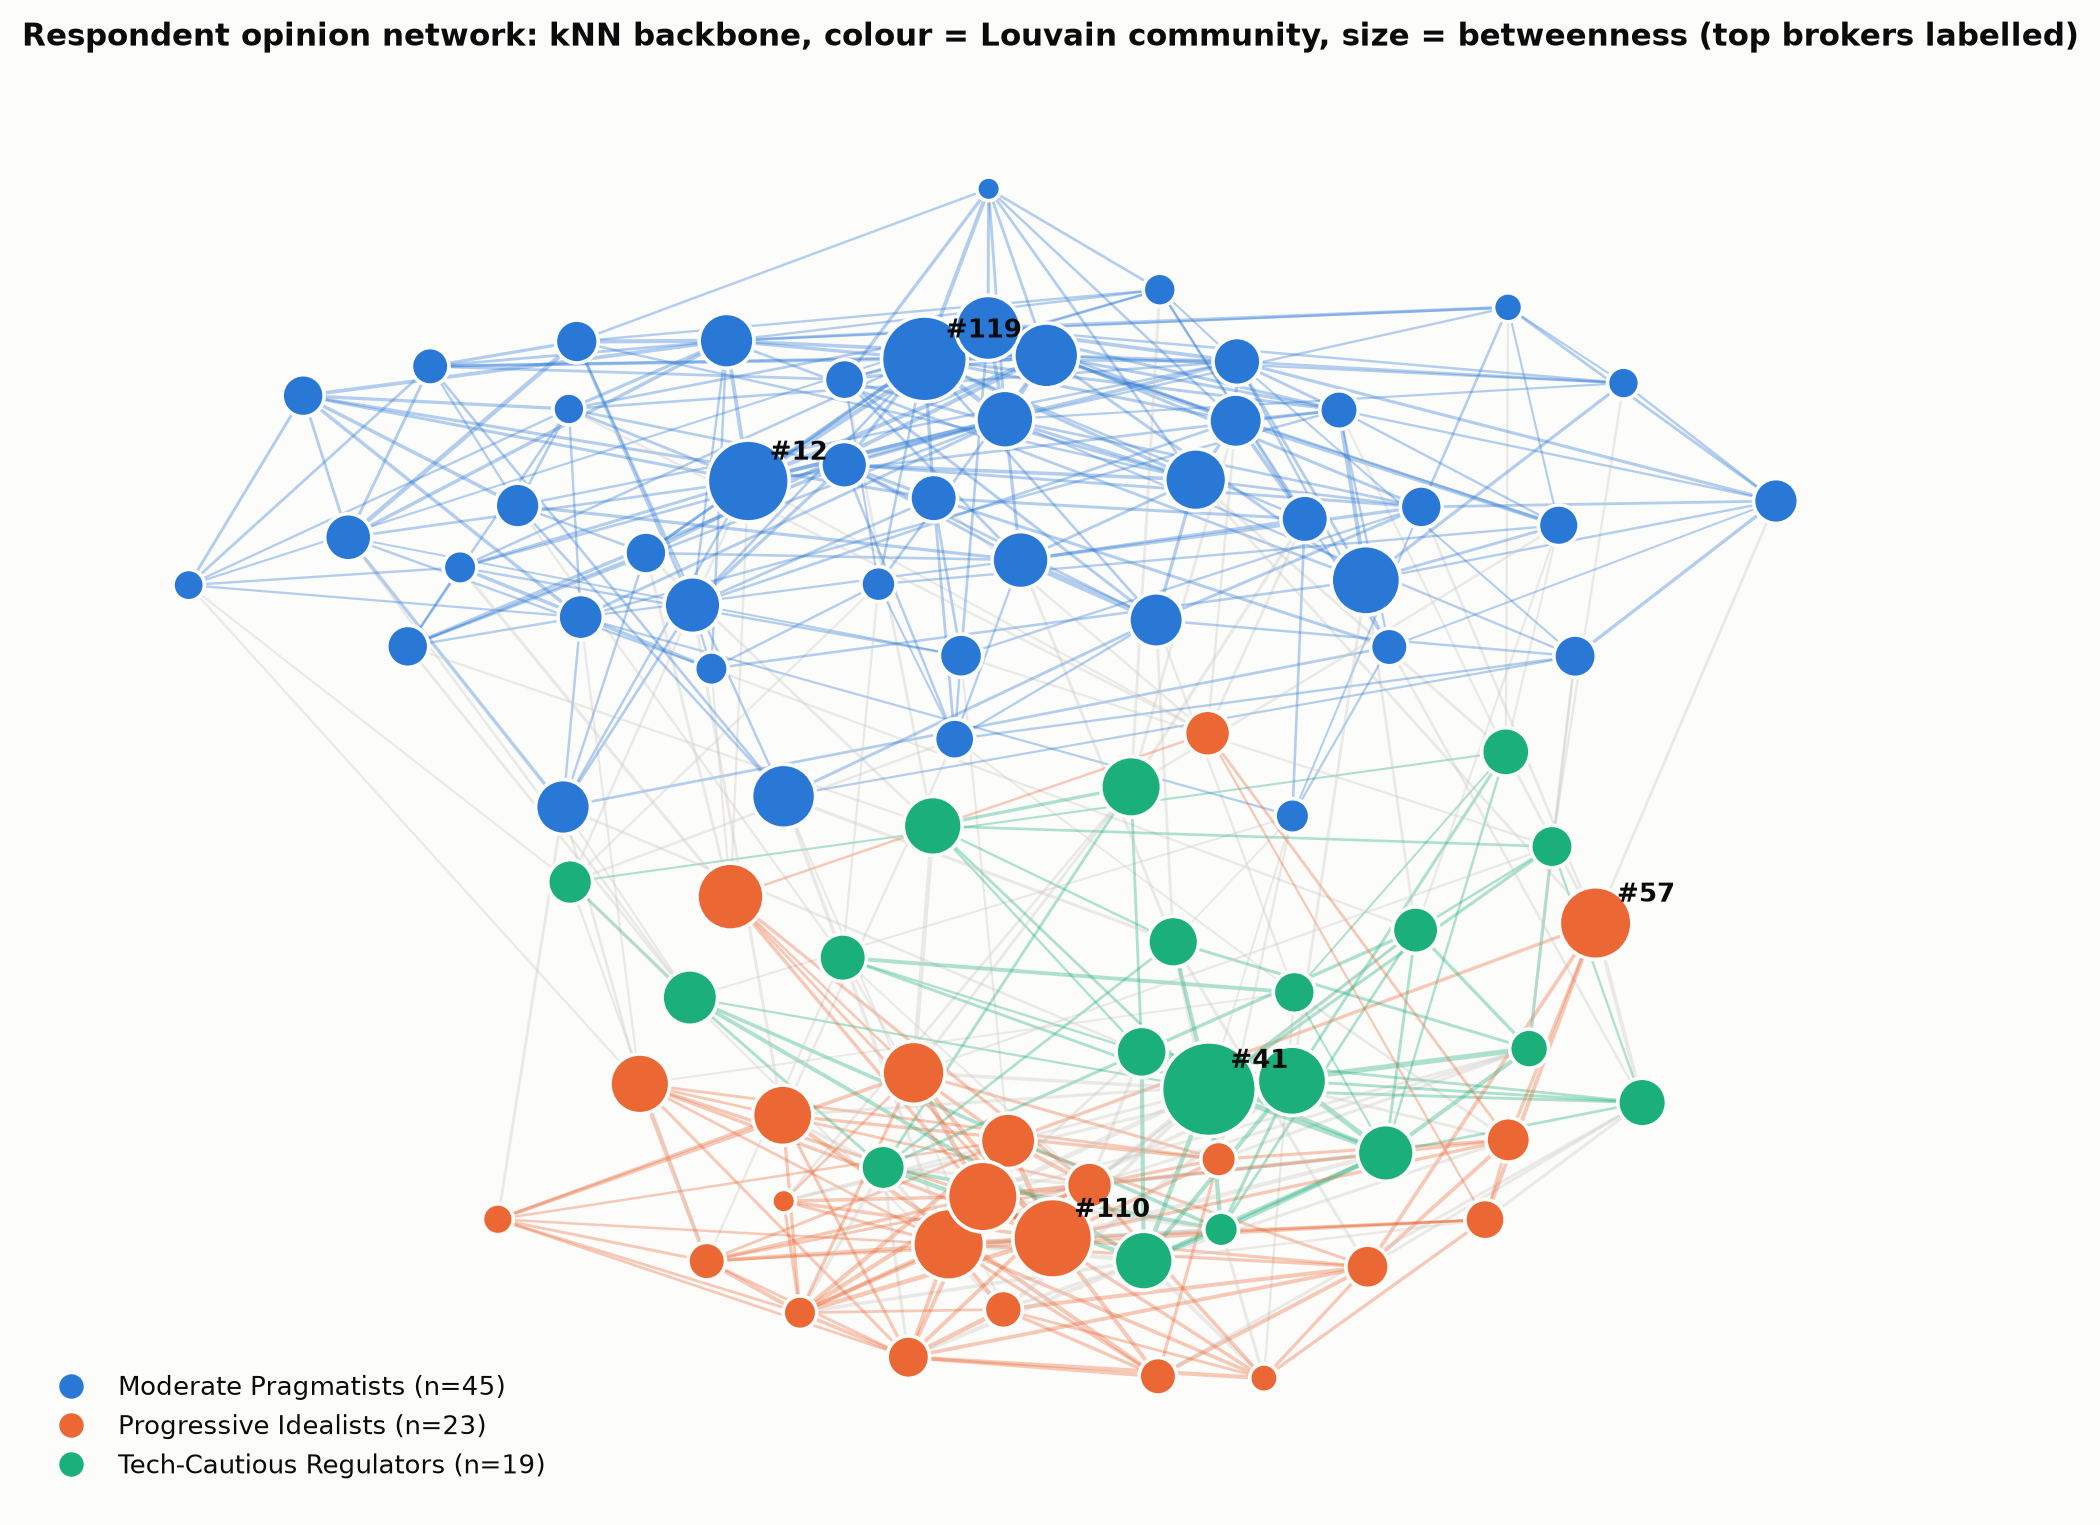
\includegraphics[width=0.84\linewidth]{fig04_respondent_network.png}
\caption{Respondent opinion network (spring layout). Node colour shows the Louvain community and size shows betweenness
centrality. Edges within a community take its colour; edges between communities are grey. \#IDs mark the five main brokers.}
\label{fig:net}
\end{figure}

\subsection{Is the community structure real?}
Modularity alone can mislead, because kNN graphs have some clustering even for random data. The column-shuffled
null model answers this directly: shuffled datasets reach $Q=0.363\pm0.014$, while the real data reaches $0.418$
($z=4.0$, empirical $p=0.005$; Fig.~\ref{fig:null}). The groups therefore reflect \emph{how individual students combine
their opinions}, not just the fact that some statements are more popular than others. Robustness checks
(\texttt{outputs/tables/construction\_robustness.csv}):
a global top-10\% threshold graph gives a nearly identical partition (ARI $=0.89$). $k=6$ and $k=10$ give finer
(5 communities) and coarser (2) versions of the same split (ARI $0.50$ / $0.65$, NMI $\approx0.6$). The resolution
sweep behaves the same way: $\gamma\le0.8$ merges the two high-agreement groups (2 communities, ARI $0.91$), and
$\gamma\ge1.2$ breaks them into less stable fragments with lower $Q$. Person-centred similarity, which removes
each student's overall tendency to agree, gives a different and weaker partition (ARI $0.17$). Part of the structure
is therefore \emph{how strongly} students agree, as the profiles below confirm.

\begin{figure}[t]
\centering
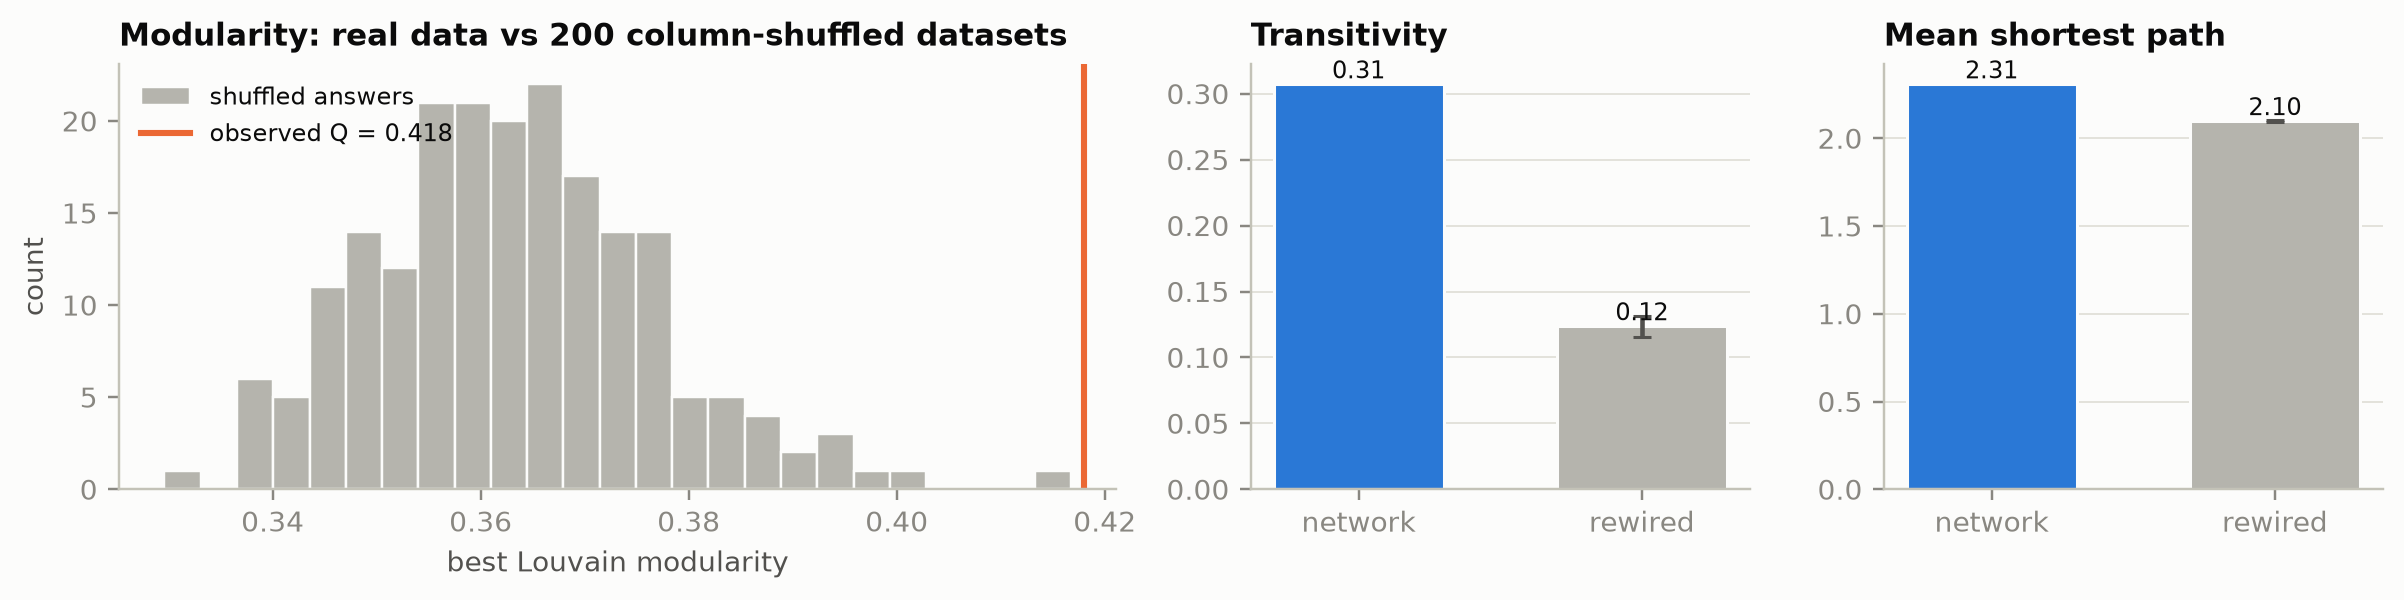
\includegraphics[width=\linewidth]{fig06_null_models.png}
\caption{Validation against null models: modularity of 200 column-shuffled datasets (left), and transitivity and
mean shortest path compared with 50 degree-preserving rewired graphs (right; error bars show 1 SD).}
\label{fig:null}
\end{figure}

\subsection{Community profiles and centrality}
\begin{figure}[t]
\centering
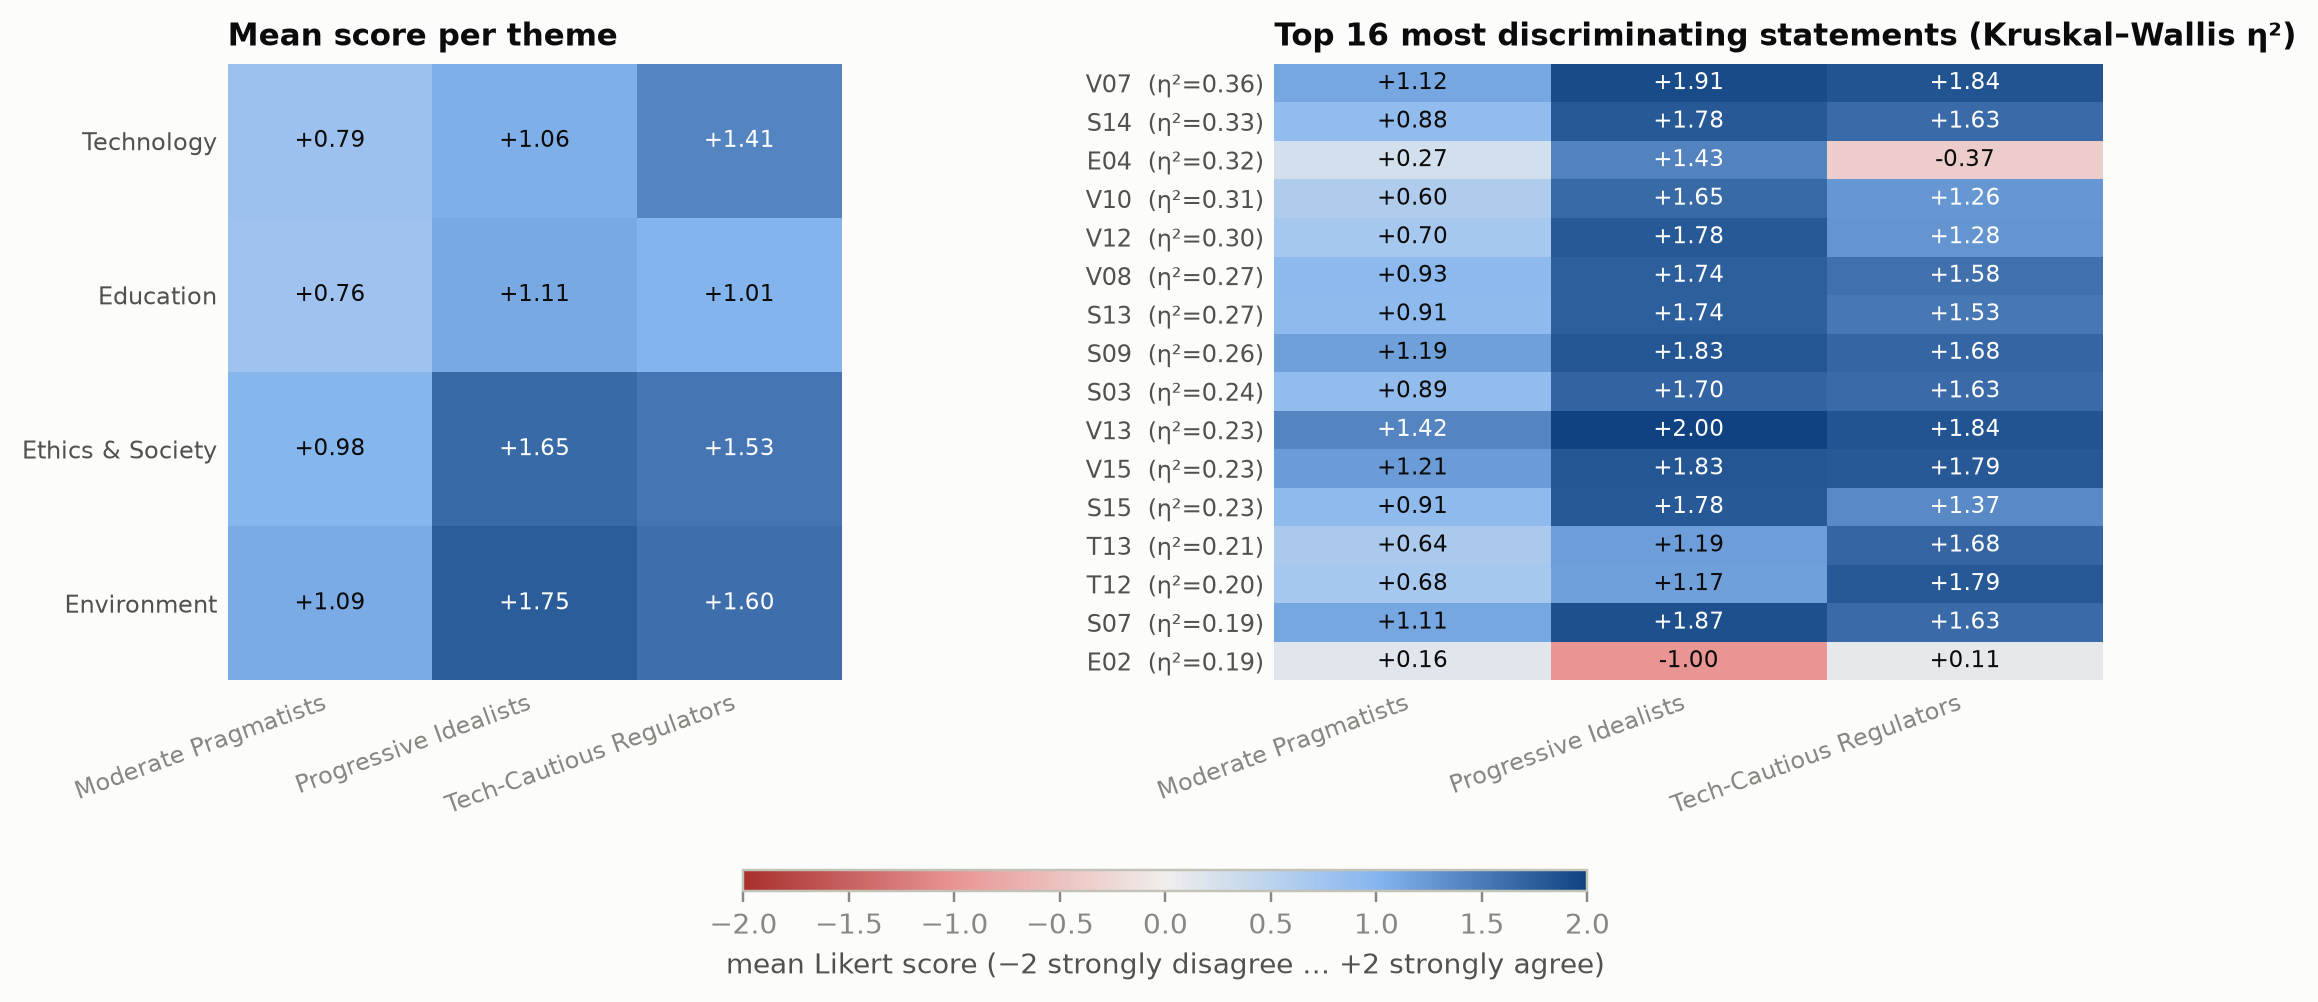
\includegraphics[width=0.95\linewidth]{fig07_community_profiles.png}
\caption{Mean score of each community per theme (left) and on the 16 statements that best separate the
communities (right, ranked by Kruskal--Wallis $\eta^2$; all $q<0.001$).}
\label{fig:profiles}
\end{figure}

\begin{figure}[t]
\centering
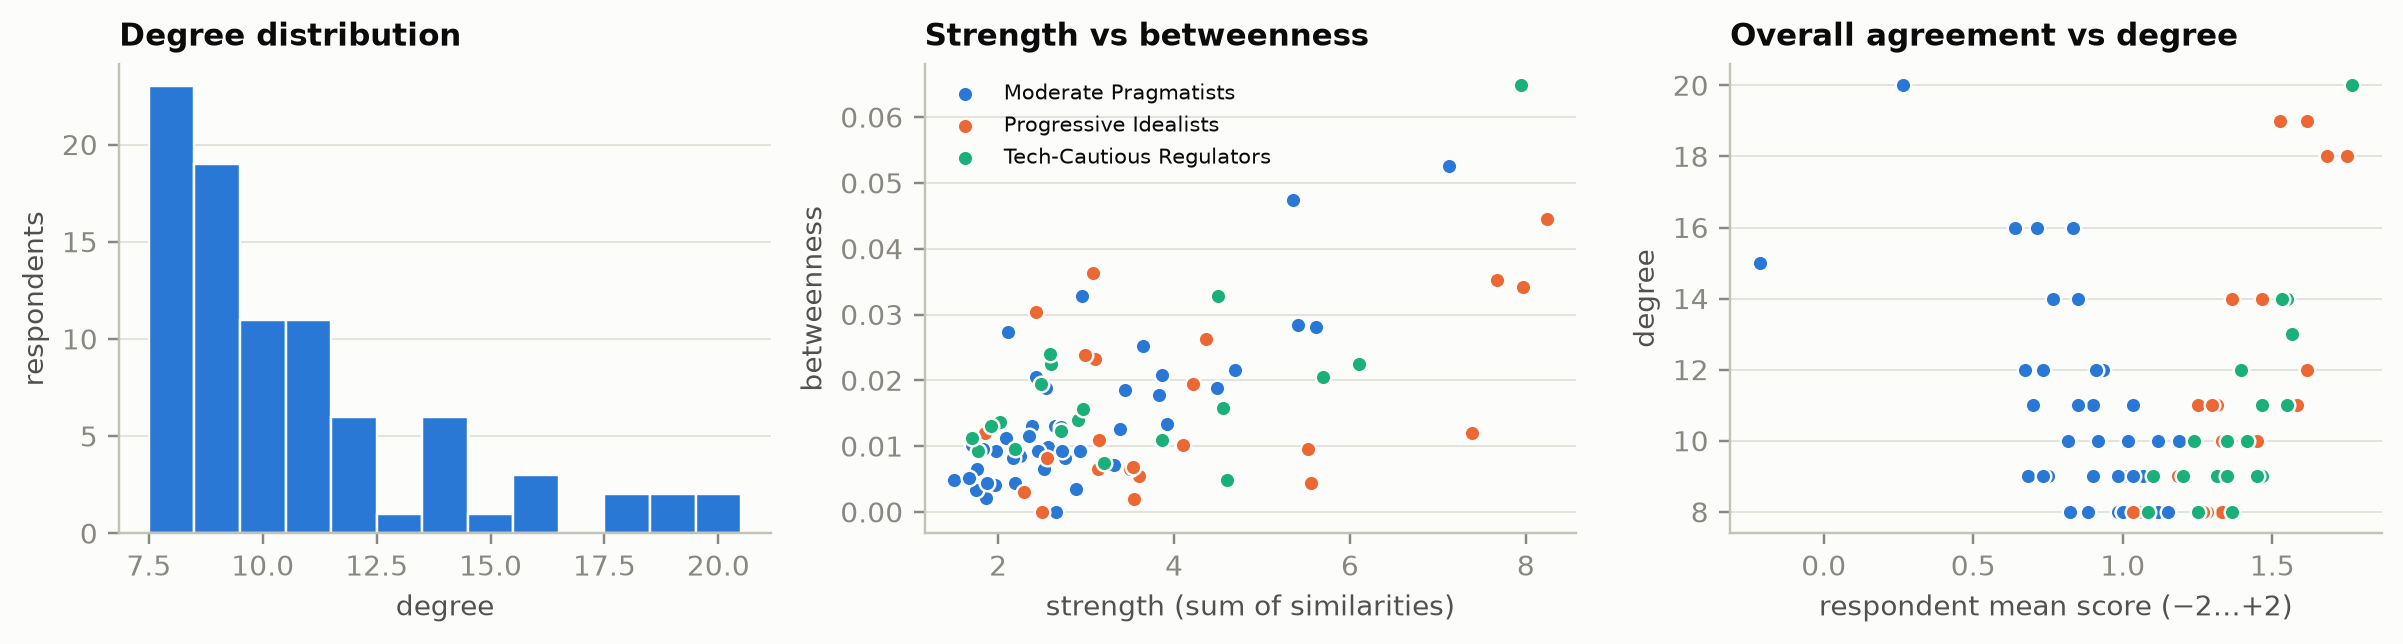
\includegraphics[width=\linewidth]{fig05_centrality.png}
\caption{Degree distribution (a kNN graph has minimum degree $k=8$), strength vs.\ betweenness, and each
respondent's overall agreement vs.\ degree.}
\label{fig:cent}
\end{figure}

The profiles (Fig.~\ref{fig:profiles}) suggest the following names for the three communities:
\begin{itemize}
\item \textbf{Moderate Pragmatists (45 students, 52\%).} They agree, but mildly: mean $+0.91$, only 27\% of answers
Strongly Agree. They are the least enthusiastic on every theme, especially the ethical and environmental ideals
(e.g.\ biodiversity V07 $+1.12$ vs.\ $\geq+1.84$ elsewhere), and neutral on online learning (E04 $+0.27$).
This is the most cohesive group: 77\% of its members' edges stay inside it.
\item \textbf{Progressive Idealists (23, 26\%).} Strongest support for environment ($+1.75$) and ethics ($+1.65$), for example
sustainable purchasing (V10 $+1.65$) and sustainability in curricula (V12 $+1.78$). They are the only group that clearly
\emph{rejects written exams as an accurate measure} (E02 $-1.00$ vs.\ $\approx+0.1$) and the most positive about
online learning (E04 $+1.43$).
\item \textbf{Tech-Cautious Regulators (19, 22\%).} Just as intense as the Idealists (59\% Strongly Agree), and the
highest Technology score of all groups ($+1.41$), driven by \emph{control} of technology: stricter AI regulation (T12 $+1.79$),
cybersecurity over new technology (T13 $+1.68$). They are the only group that on average \emph{disagrees} that online learning can
complement classroom teaching (E04 $-0.37$). Only 37\% of their edges are internal, so they sit between the other two groups.
\end{itemize}
Eleven statements do \emph{not} differ between groups ($q>0.05$). These include academic honesty (E08), whether AI improves society (T01),
autonomous vehicles (T09), social-media polarisation (T14) and control over personal data (S05). These opinions are shared across the
whole class (S05, E08) or remain mixed inside every group (T01, T09).

\textbf{Centrality.} The main brokers (Fig.~\ref{fig:net}) are \#41 (Regulator; degree 20, betweenness 0.065),
\#119 and \#12 (Pragmatists) and \#110, \#57 (Idealists). Centrality is almost unrelated to overall agreement
(Spearman $\rho$: degree $0.14$, betweenness $0.06$; Fig.~\ref{fig:cent}). Well-connected students are not simply the most
agreeable. For example, \#119 has one of the lowest mean scores ($+0.27$) yet the highest degree, because many
moderate students deviate from the class average in the same way.

\subsection{Per-theme networks}
\begin{figure}[h]
\centering
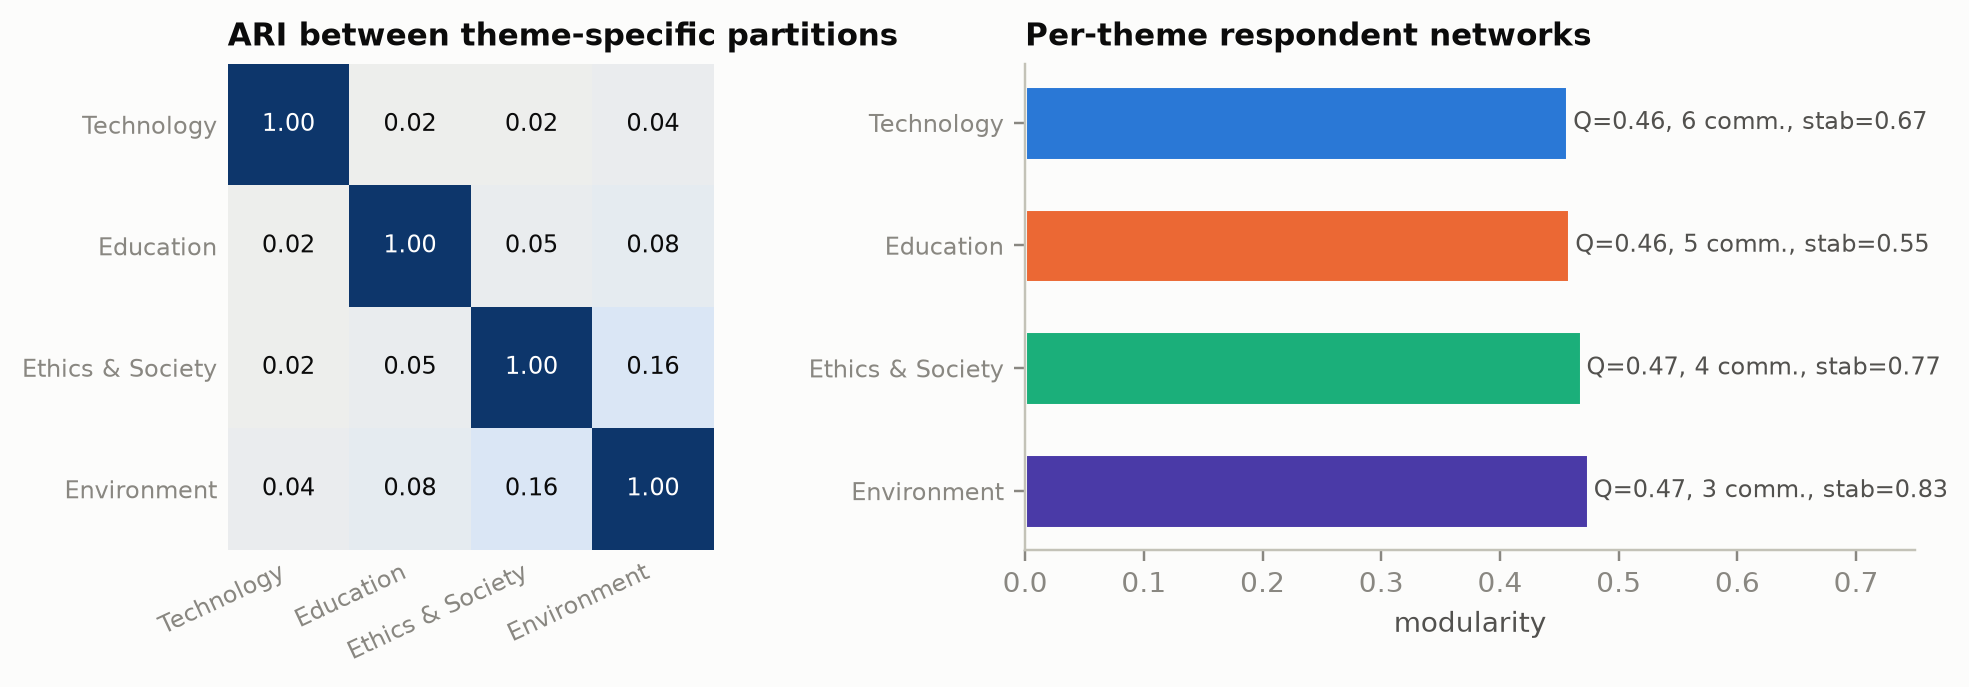
\includegraphics[width=0.8\linewidth]{fig08_theme_networks.png}
\caption{Left: agreement (ARI) between the communities found separately from each theme's 15 statements.
Right: modularity, community count and seed stability of each per-theme network.}
\label{fig:themes}
\end{figure}
Each single-theme network has clear communities ($Q=0.46$--$0.47$), but the partitions barely overlap across themes
(ARI $0.02$--$0.16$, Fig.~\ref{fig:themes}). Students who group together on Technology are essentially a random mix on
Education. The only noticeable overlap is between Ethics \& Society and Environment (0.16). Environment gives the
cleanest and most stable split (3 communities, stability 0.83), and Education the least stable (0.55).

\subsection{Statement network}
\begin{figure}[t]
\centering
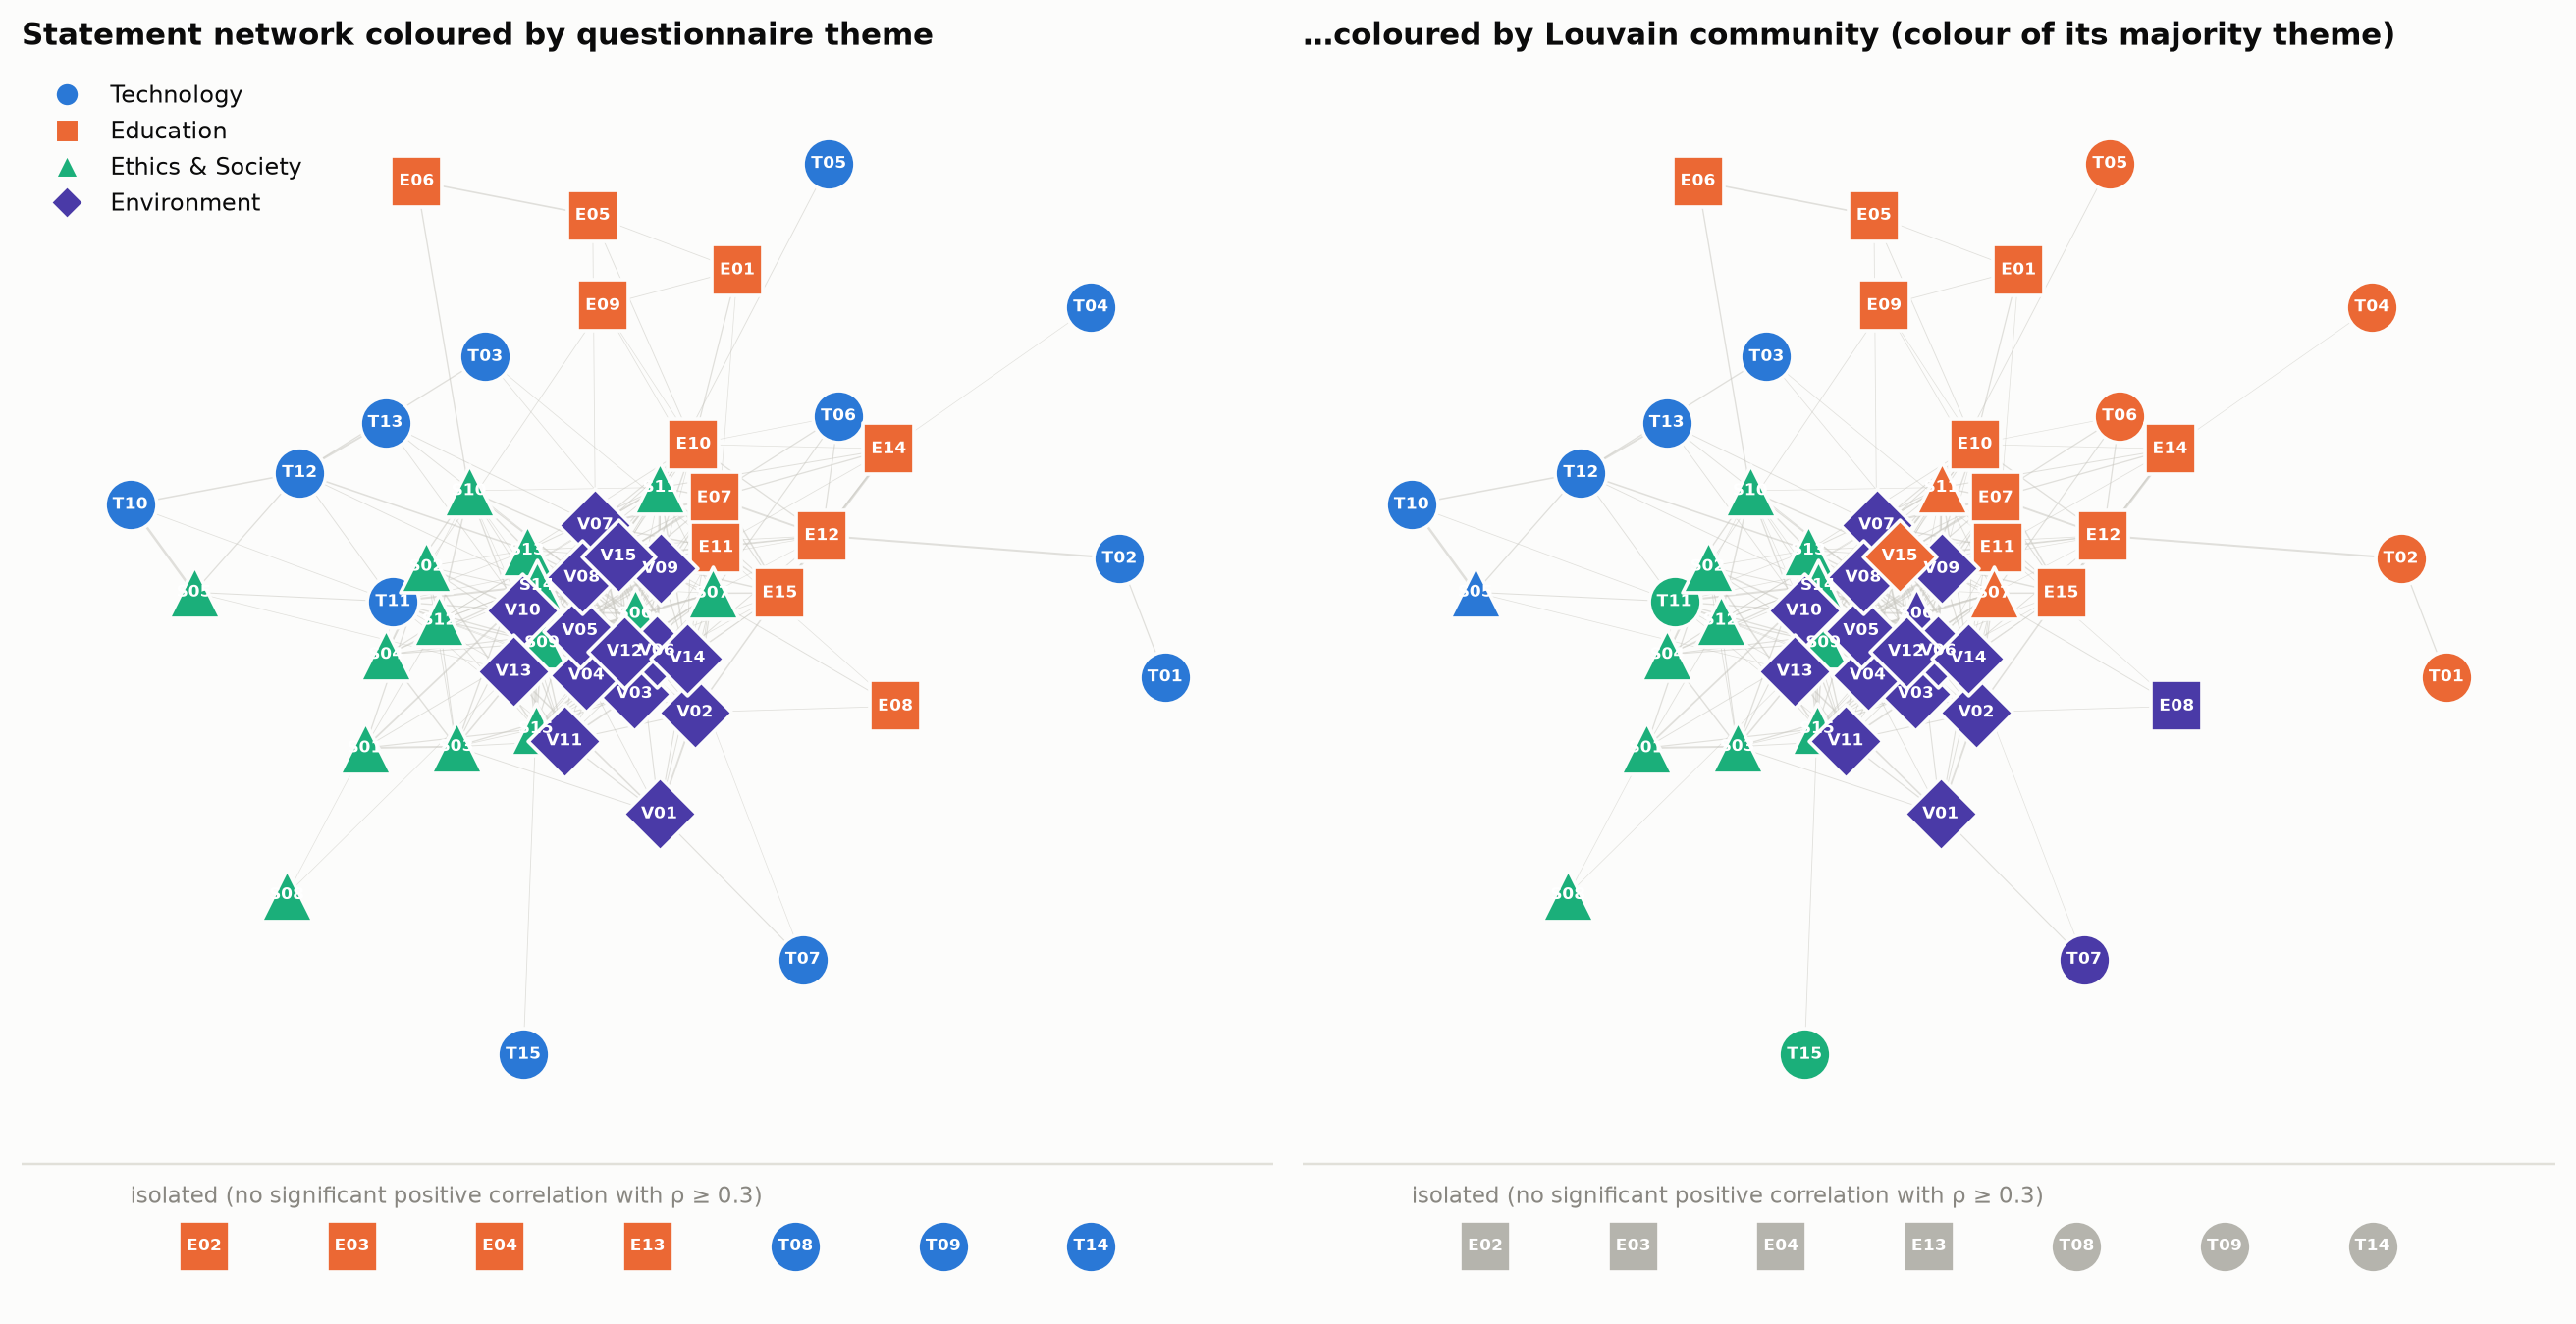
\includegraphics[width=\linewidth]{fig09_item_network.png}
\caption{Statement network (FDR $q<0.05$, $\rho\geq0.30$). Left: coloured by questionnaire theme (marker shape
also shows the theme). Right: coloured by detected community; a node whose colour differs from its shape's theme
belongs to a community dominated by another theme. The bottom strip lists the 7 statements with no qualifying edge.}
\label{fig:items}
\end{figure}

The statement network has 321 edges. The 53 connected statements form one component with high clustering
(transitivity 0.55, mean path 2.12). The strongest links are all within Environment (V07--V08 $\rho=0.65$, V08--V10 $0.63$,
V05--V07 $0.59$). Correlations are higher within a theme than between themes (mean $\rho$ 0.22 vs.\ 0.13), and Louvain
($Q=0.24$, stability 0.86) partly recovers the questionnaire design (NMI $=0.47$, ARI $=0.39$), with four meaningful communities:
\begin{enumerate}
\item \textbf{Environment} (17): V01--V14 plus academic honesty (E08), shared responsibility against misinformation (S06) and robots in hazardous jobs (T07).
\item \textbf{Civic ethics} (13): most S-statements plus explainable recommendation algorithms (T11) and dependence on AI decision-making (T15).
\item \textbf{Modern, tech-enabled learning} (18): E01, E05--E07, E09--E12, E14--E15 \emph{together with the optimistic AI
statements} T01, T02, T04, T05, T06, as well as S07, S11 and V15. Support for AI and support for modern teaching are one attitude.
\item \textbf{Digital rights \& regulation} (5): disclosure of AI use (T03), data over convenience (T10), stricter AI regulation (T12),
cybersecurity investment (T13) and control of personal data (S05). This group cuts across themes and corresponds to the
opinions that define the Tech-Cautious Regulators.
\end{enumerate}
The \textbf{7 isolated statements} (E02, E03, E04, E13, T08, T09, T14) include the four least consensual statements
(E04, E02, E03, T08). Opinions on them are independent of the rest of a student's views. T14 (polarisation) is the
exception: so many students strongly agree with it that its answers vary too little to correlate with anything. The few significant \emph{negative}
correlations all involve traditional teaching: support for compulsory attendance (E03) goes with \emph{less} support for innovation over rote
learning (E10, $\rho=-0.40$), updated curricula (E11, $-0.35$) and AI in teaching (E12, $-0.30$). Belief in written exams
(E02) goes against project-based learning (E01, $-0.33$). The statements with the highest weighted degree are
inclusive discussion (S09), ethical leadership (S14) and biodiversity (V07). Those with the highest betweenness,
AI in teaching (E12) and S09/S14, link the learning, ethics and environment clusters.

%==============================================================================================
\section{Results and Discussion}
\begin{enumerate}[leftmargin=1.3em]
\item \textbf{A class with high consensus on values and real disagreement about teaching and AI in practice.}
Almost 80\% of answers agree, and the most consensual views are about values: lifelong learning, corporate and
environmental accountability, data rights. Real disagreement is limited to a few concrete questions: exams,
attendance, online learning, AI in healthcare and autonomous vehicles. Most of these divisive statements are also
isolated in the statement network, so they are \emph{separate} questions rather than symptoms of a general worldview.

\item \textbf{Three opinion groups, confirmed against a null model.} Similarity between students forms a
small-world network with three communities ($Q=0.418$, well above the $0.363\pm0.014$ of shuffled data). The largest
group, the Moderate Pragmatists (about half the class), differs from the rest mainly in \emph{intensity}: the same direction
of opinion, weaker conviction. The other two groups are equally intense but differ in \emph{content}.
Progressive Idealists put sustainability first and reject exam-based assessment. Tech-Cautious Regulators
put regulation and security of technology first and doubt online learning. The difference between these two groups is
the clearest ``ideological'' divide in the class.

\item \textbf{Opinions are organised by attitude, not only by topic.} The statement network recovers the survey's
themes only partly (NMI 0.47). AI optimism merges with modern-pedagogy views, and a small cross-theme
\emph{digital-rights} cluster (privacy, regulation, AI disclosure, cybersecurity) appears. The class does not treat
``technology'' as one topic: students separate \emph{using} AI (a learning question) from \emph{governing} it (a
rights question).

\item \textbf{Groups are topic-specific.} Grouping students by one theme says almost nothing about how they group on
another (ARI $\le0.16$). Only ethics and environment are somewhat aligned. Students form different alliances
on different subjects, and the overall three-group structure mainly reflects the ethics/environment axis and
the regulation/online-learning split.

\item \textbf{Bridges and brokers.} The Tech-Cautious Regulators group is the least self-contained (37\% internal edges)
and holds the highest-betweenness student (\#41), so it links the two more cohesive groups. Centrality does not
depend on overall agreement: central students are \emph{typical} of a shared deviation from the class average,
not simply the most enthusiastic.
\end{enumerate}

\textbf{Limitations.} (i) With 87 respondents the finer structure is uncertain: stability is 0.74 and nearby
choices of $k$ or resolution split or merge the two high-agreement groups, although the Pragmatist-vs-rest divide holds throughout.
(ii) Part of the respondent structure reflects response style (how strongly students agree); person-centred similarity, which removes
it, gives a weaker partition. We present both readings instead of choosing one. (iii) Likert answers are ordinal; cosine
similarity treats them as interval, while Spearman (statement network) and Kruskal--Wallis (profiling) do not.
(iv) The survey is a single cross-section with no demographic data, so the groups cannot be linked to programme or year.

%==============================================================================================
\section{Individual Contribution}
The specific tasks completed by each member are listed below. Each member also reviewed the others' code and the final report.

\begin{table}[h]
\centering\small
\begin{tabularx}{\linewidth}{@{}p{2.3cm}X@{}}
\toprule
\textbf{Member} & \textbf{Specific tasks completed}\\
\midrule
\textbf{Inesh} &
\textbf{Project lead and network design.} Designed the overall two-network approach. Chose and implemented the
item-centred, pairwise-complete cosine similarity and the kNN backbone (\texttt{src/network.py}), including the
$k$-sweep used to select $k=8$. Implemented Louvain community detection with multi-seed stability, the resolution
sweep, the column-permutation null model, the degree-preserving small-world test and the construction-robustness
comparison (\texttt{src/analysis.py}). Built the end-to-end pipeline (\texttt{run\_pipeline.py}), set up and organised the
GitHub repository, interpreted the three opinion communities and wrote the Pipeline, Results \& Discussion and
Limitations sections.\\
\midrule
\textbf{Khwaish} &
\textbf{Data preparation and opinion profiling.} Studied the survey structure and wrote the loading and encoding
module (\texttt{src/preprocess.py}): Likert coding, treating ``No Comments'' as missing, respondent quality
diagnostics, the 75\% completeness filter, and checks for straight-lining and duplicate responses. Produced the
descriptive statistics and the Tastle--Wierman consensus analysis, implemented the Kruskal--Wallis/FDR community
profiling, and created Figures 1 and 5. Wrote the Dataset Documentation section and the community profile descriptions.\\
\midrule
\textbf{Hiten} &
\textbf{Statement network, centrality and visualisation.} Implemented the Spearman correlation matrix with
Benjamini--Hochberg filtering, built the statement network and evaluated its communities against the themes (NMI/ARI).
Built the per-theme respondent networks and the cross-theme ARI comparison, and computed the node centralities and
broker analysis. Wrote the plotting module (\texttt{src/visualize.py}) with a colour-blind-checked palette and created
Figures 2--4 and 6--8 (plus the correlation heatmap in the repository). Wrote the README and requirements for reproducibility, wrote the statement-network analysis
section and formatted the final report.\\
\bottomrule
\end{tabularx}
\end{table}

\end{document}
